%!TEX root=../document.tex

\section{Source-Code}
\subsection{JDBCClient.java}
\begin{lstlisting}[language=Java]
package webshop;


import java.sql.Connection;
import java.sql.DriverManager;
import java.sql.PreparedStatement;
import java.sql.ResultSet;
import java.sql.SQLException;
import java.sql.Statement;
import java.util.ArrayList;
import java.util.List;

public class JDBCClient {
	
	Connection con;
	
	JDBCClient() throws SQLException{
		//Initialize the connection with test user that has priviliges
		this.con = DriverManager.getConnection("jdbc:postgresql://localhost:5432/webshop","test","test");
	}
	/***
	* Makes an preparedStatemenent and then fills and ArrayList with Artikel
	* @return List of all articles
	* @throws SQLException
	*/
	List<Artikel> getAllArticles() throws SQLException {
		PreparedStatement pstmt = con.prepareStatement("SELECT * FROM artikel");
		ResultSet rs = pstmt.executeQuery();
	
		ArrayList<Artikel> rl = new ArrayList<>();
		while(rs.next()){
			int anr = rs.getInt("anr");
			String abez = rs.getString("abez");
			String ainfo = rs.getString("info");
			Float preis = rs.getFloat("npreis");
			int vstueckz = rs.getInt("vstueckz");
			rl.add(new Artikel(anr,abez,ainfo,preis,vstueckz));
		}
		return rl;
	}
	
	/***
	* Makes an preparedStatement and then inserts the desired article into the database with executeUpdate()
	* @param a the desired article to be inserted into the database
	* @throws SQLException
	*/
	void addArticle(Artikel a) throws SQLException {
		PreparedStatement ptsmt = con.prepareStatement("INSERT INTO artikel(anr,abez,npreis,vstueckz,info) values(?,?,?,?,?)");
		ptsmt.setInt(1, a.getAnr());
		ptsmt.setString(2, a.getAbez());
		ptsmt.setFloat(3, a.getPreis());
		ptsmt.setInt(4, a.getVstueckz());
		ptsmt.setString(5, a.getAinfo());
		ptsmt.executeUpdate();
	}
	
	/**
	* Makes an preparedStatement and then updates the desired article with the values
	* @param a the article to be updated
	* @throws SQLException
	*/
	void saveArticle(Artikel a) throws SQLException {
		PreparedStatement ptsmt = con.prepareStatement("UPDATE artikel SET anr=?,abez=?,npreis=?,vstueckz=?,info=? WHERE anr=?");
		ptsmt.setInt(1, a.getAnr());
		ptsmt.setString(2, a.getAbez());
		ptsmt.setFloat(3, a.getPreis());
		ptsmt.setInt(4, a.getVstueckz());
		ptsmt.setString(5, a.getAinfo());
		ptsmt.setInt(6, a.getAnr());
		ptsmt.executeUpdate();
	}
	
	/**
	* Delete an article based on the primary key anr
	* @param anr primary key which defines an article so it can be deleted
	* @throws SQLException
	*/
	void delArticle(int anr) throws SQLException{
		PreparedStatement ptsmt = con.prepareStatement("DELETE FROM artikel WHERE anr=?");
		ptsmt.setInt(1, anr);
		ptsmt.executeUpdate();
	}
}
\end{lstlisting}

\subsection{ArtikelAdmin.java}
Hier wurde lediglich ein löschen Button hinzugefügt welcher nur auf das \verb|anr| input-Feld zugreift. Wenn der Button gedrückt wird, wird jedoch auch aus der Liste welche alle in der GUI vorhandenen Artikel besitzt der gewünschte mit der anr definierten Nummer Artikel aus der Liste genommen:

\begin{lstlisting}[language=Java]
final Button delButton = new Button("Loeschen");
delButton.setOnAction(new EventHandler<ActionEvent>() {
	@Override
	public void handle(ActionEvent e) {
		int anr = Integer.parseInt(addAnr.getText());
		for(int i = 0; i < data.size(); i++){
			if(data.get(i).getAnr() == anr){
				data.remove(i);
			}
		}
		try {
			db.delArticle(anr);
		} catch (SQLException e1) {
			e1.printStackTrace();
		}
		addAnr.clear();
	}
});
\end{lstlisting}

Und dieser Button muss noch hinzugefügt werden zu der GUI

\begin{lstlisting}[language=Java]
hb.getChildren().addAll(addAnr, addAbez, addAinfo, addPreis, addVstueckz, addButton,delButton);
\end{lstlisting}

\section{Screenshots}
\subsection{GUI}
\begin{minipage}{\linewidth}
	\centering
	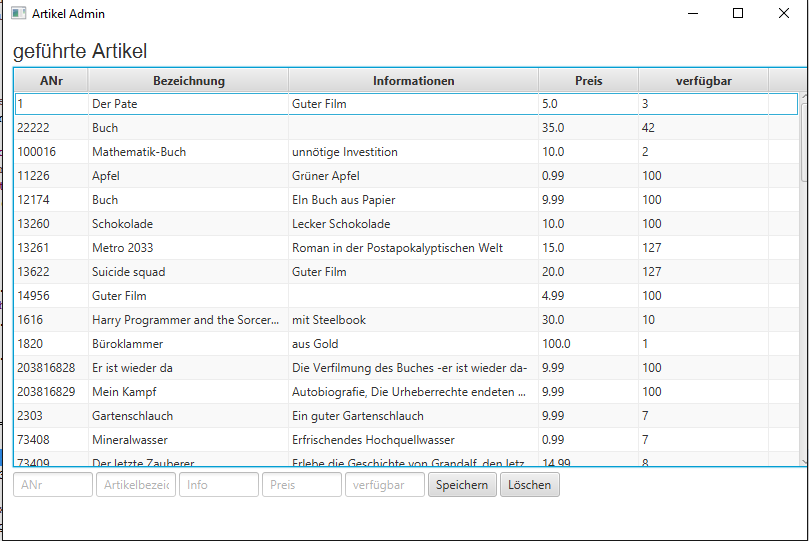
\includegraphics[width=0.8\linewidth]{images/gui}
	\figcaption{Alle Artikel werden angezeigt}
\end{minipage}

\subsection{Artikel hinzufügen}

\begin{minipage}{\linewidth}
	\centering
	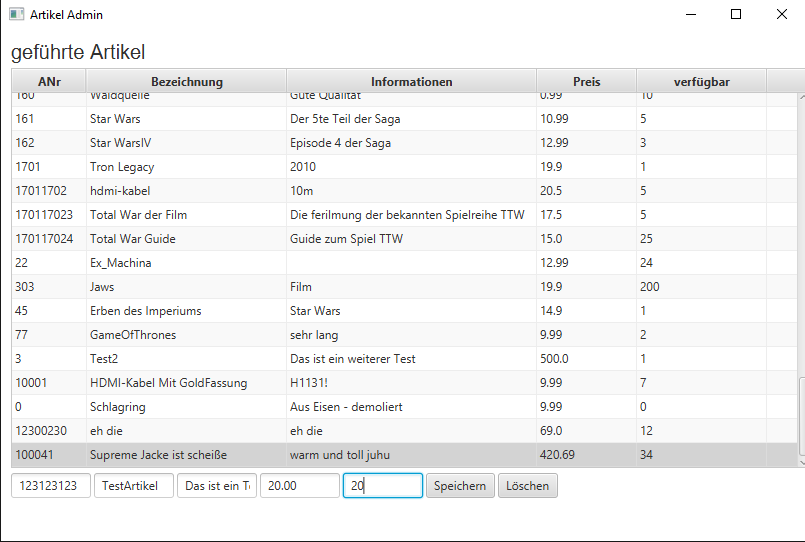
\includegraphics[width=0.8\linewidth]{images/hinzufuegen1}
	\figcaption{Artikelinformationen werden eingetragen}
\end{minipage}

\begin{minipage}{\linewidth}
	\centering
	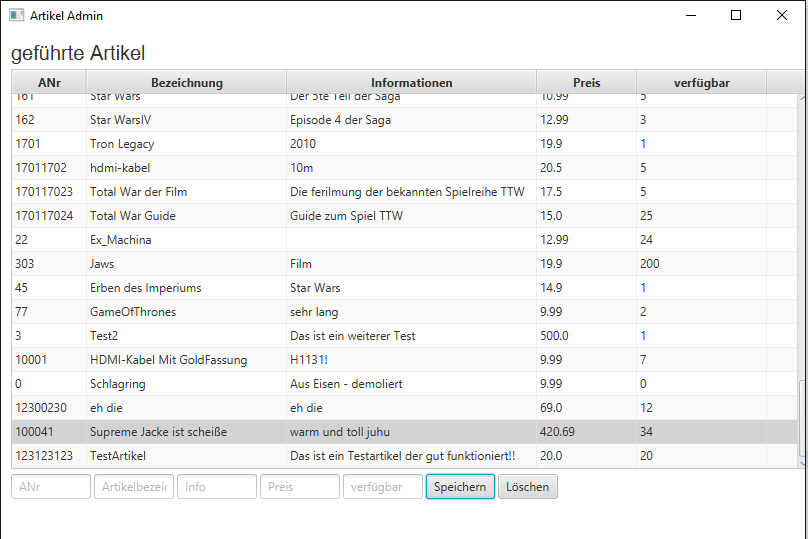
\includegraphics[width=0.8\linewidth]{images/hinzufuegen2}
	\figcaption{Artikel wurde hinzugefügt}
\end{minipage}

\subsection{Artikel ändern}

\begin{minipage}{\linewidth}
	\centering
	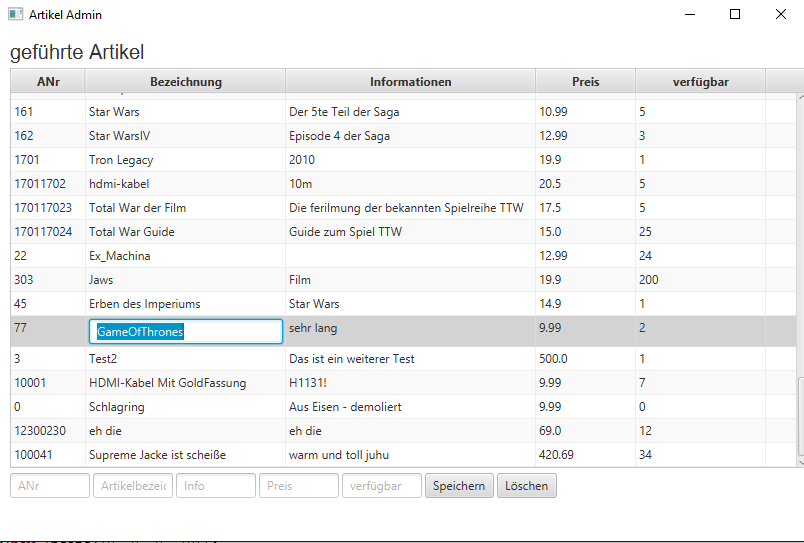
\includegraphics[width=0.8\linewidth]{images/aendern1}
	\figcaption{Artikelinformationen werden bearbeitet}
\end{minipage}

\begin{minipage}{\linewidth}
	\centering
	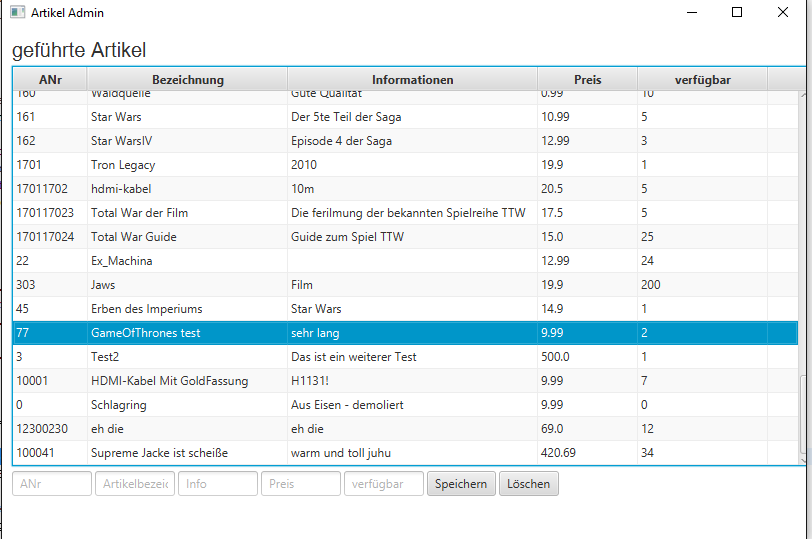
\includegraphics[width=0.8\linewidth]{images/aendern2}
	\figcaption{Artikel wurde geändert}
\end{minipage}

\begin{minipage}{\linewidth}
	\centering
	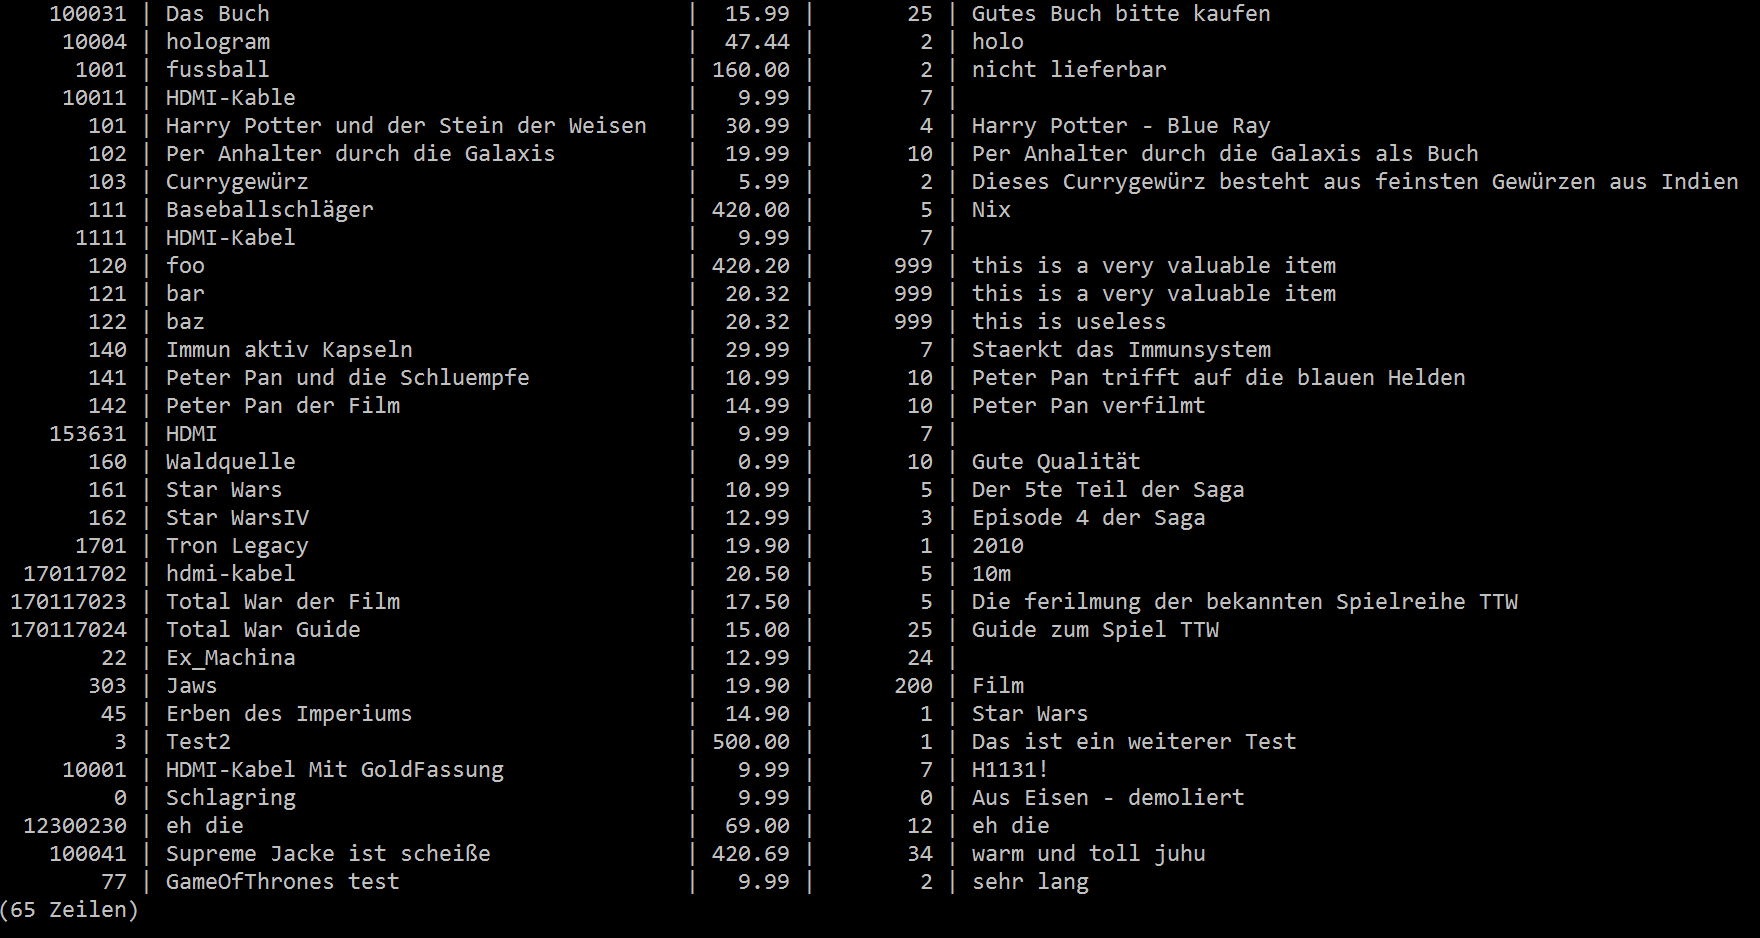
\includegraphics[width=0.8\linewidth]{images/aendern3}
	\figcaption{Auch in der Datenbank}
\end{minipage}

\subsection{Artikel löschen}
\begin{minipage}{\linewidth}
	\centering
	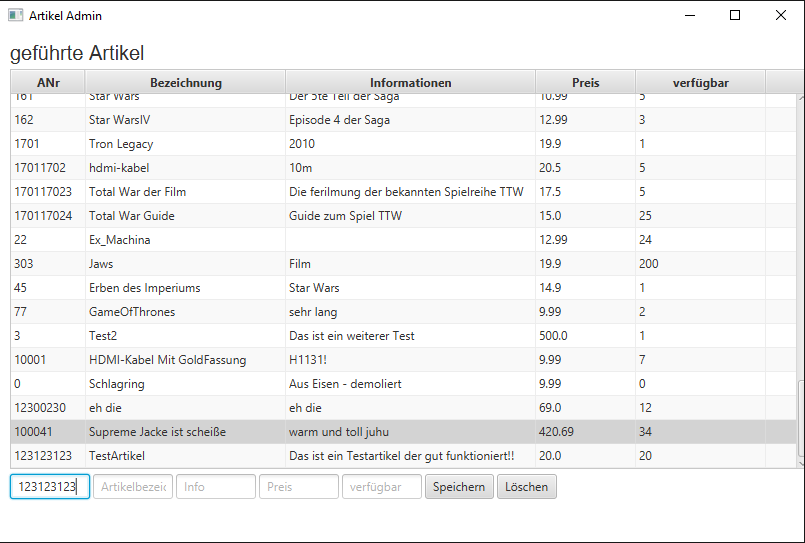
\includegraphics[width=0.8\linewidth]{images/loeschen1}
	\figcaption{anr wird eingegeben zum löschen des Artikels}
\end{minipage}

\begin{minipage}{\linewidth}
	\centering
	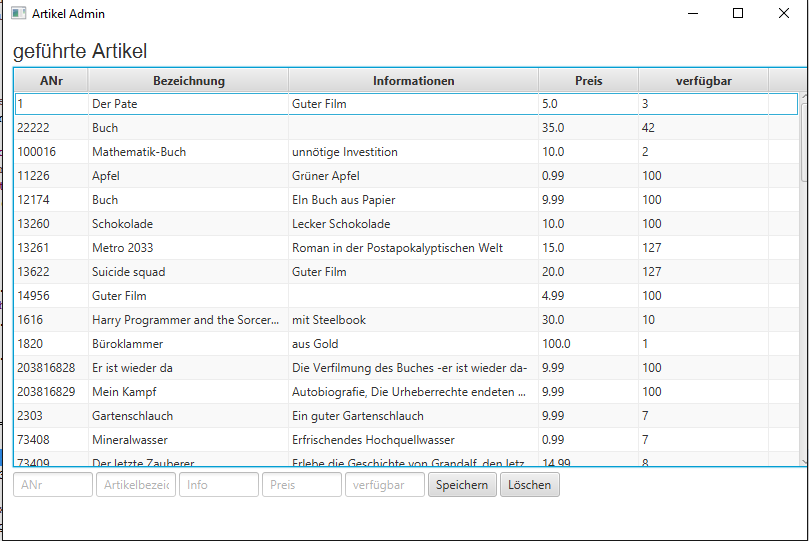
\includegraphics[width=0.8\linewidth]{images/gui}
	\figcaption{Artikel wurde anhand der anr gelöscht}
\end{minipage}


\section{SQL Injection}
Beispiel:

Passworteingabe funtkioniert über input Feld welches simpel in Klartext ein Wort übernimmt und ihn der Datenbank überprüft ob es mit dem Passwort dort übereinstimmt. Annahme: \textbf{Keine PreparedStatements!}

Um nun diese Eingabe sehr leicht überbrücken zu können muss man jediglich folgendes eingeben: \verb|'' OR 1=1|

Was es bewirkt:
In der Überprüfung steht etwas in der Art wie:\\
\verb|SELECT ... FROM ... WHERE pwd = pwd;|.

Nun wenn man etwas wie oben beschrieben eingibt ergibt sich folgender SQL Query:
\\
\verb|SELECT ... FROM ... WHERE pwd = '' OR 1=1;|

Was dazu führt dass das Passwort immer richtig ist.


PreparedStatements funktionieren indem diese genau wissen welche Werte sie entgegen nehmen werden, z.B. werden dann wenn die Eingabe ein String ist, wird wirklich die Eingabe wie ein String behandelt und nicht wie ein SQL Statement
